% =====================================================================
% Data section: working draft v2 (Claude, 18 Oct 2026)
% ---------------------------------------------------------------------
% Toon asked (18 Oct) for a full draft of what goes in the manuscript.
% Markup, delete before submission:
%  * \draftnum{}   number NOT yet verified against the papers (orange). Numbers without
%                  this macro were checked against the PDFs on 18 Oct 2026 (Claude, counted
%                  as verified by Toon's decision; see out/verified_*.csv). Replace with values from
%                  build/analyse_dataset_usage.py `sheet` mode or rows with page_ref.
%  * \claudedraft{} sentence that interprets or argues (blue). Claude wrote it so
%                  the section reads end to end; the supervisor requires the
%                  interpretation to be Toon's own, so rewrite or delete every one.
%  * \evidence{}   where the numbers come from (grey). Delete in the final version.
%  * \pcite{}      placeholder for a bibliography key not yet in references.bib.
% Sources: out/full_summary.json, out/full_outcome_rows.csv, out/full_datasets.csv
% (72 papers re-read 18 Oct with table and page refs), out/data_handling_summary.json
% (selection-rationale codes, 6 Oct records), handoff.md.
% No em-dash anywhere. Placement in main.tex undecided (new file vs 07).
% Revised 28 Oct 2026 (Claude, Toon asked): new subsection "How Difficult Are the
% Datasets That Can Be Checked?" (sec:data-difficulty, tab:data-difficulty,
% fig:data-difficulty) from Data section/difficulty/; new keys napierala2016types,
% wilson1997improved, jain2000statistical, fernandez2008study (entries in
% difficulty/difficulty_refs.bib, not yet in references.bib). Figure file:
% manuscript/figures/data-difficulty.pdf (copy to the repo figures/ folder on merge).
% Revised 19 Oct 2026 (Claude, approved by Toon): counts reconciled with
% build/reconcile_counts.py (out/reconcile_counts.json, rules R1-R6). Tomek links
% placeholder excluded from name counts; KNNOR's mean reported apart from the
% per-dataset set (541 rows, 30 papers); RBBoost's cross-table pairs excluded
% from every comparison set. See handoff.md, entries of 19 Oct.
% Conventions followed (from the repo README, main.tex, tables/ and Section 7):
%  * British spelling, as in P's Section 7 draft (normalise, binarise, analyse).
%  * Section and caption titles in Title Case; caption above the table;
%    booktabs rules with \midrule only between header and body.
%  * \pcite{key} uses the bibkeys of P's Section 7 (out/section7_key_map.csv); all 43 keys now have
%    entries in manuscript/data-section-refs.bib (Crossref-checked, 28 Oct 2026); tested by compiling main.tex
%    with every \pcite turned into \parencite: no undefined citation;
%    switch to \parencite / \textcite once the entries are in references.bib.
%  * Counts: corpus 76 papers; 73 have an evaluation on data (ENN, AdaBoost and
%    Pradipta et al. excluded; Tomek links counted by Toon's decision 18 Oct).
%    P's Section 7 counts 71 empirical studies: it excludes Tomek links and also
%    treats Hassanat et al. 2022 as a survey. State both numbers when the sections meet.
%  * Data-type labels: original / repository-defined (kept separate, Toon 23:34) /
%    modified / synthetic / not stated. Win, tie, loss: interim rule A of
%    decisions-pending (Toon 18 Oct), pending the supervisor.
% Overlap with P's Section 7 draft (section07-empirical-comparisons-draft.html),
% left as is here; to settle with P before merging:
%  * Extraction Procedure  ~ Sec 7 "Corpus and Coding Scheme" and Sec 3.3
%  * Benchmark Landscape    ~ Sec 7 "Benchmark Data (RQ1)" (UCI/KEEL shares,
%                              datasets per study, synthetic data)
%  * Recommendations item 6 ~ Sec 7 RQ4 (tuning) and RQ2 (baselines), and
%                              Sec 7 "A Minimum Evaluation Standard" (tab-remedies)
% =====================================================================
% booktabs is loaded by acmart/jair.cls; the preview wrapper must load it too.
\providecommand{\draftnum}[1]{\textcolor{orange}{#1}}
\providecommand{\claudedraft}[1]{\textcolor{blue}{#1}}
\providecommand{\evidence}[1]{\par\noindent{\footnotesize\textcolor{gray}{\textbf{Evidence:} #1}}\par}
\providecommand{\pcite}[1]{[\textsc{#1}]}
\providecommand{\Description}[1]{}% acmart/jair define it; the preview wrapper does not
\providecommand{\toon}[1]{\par\noindent\fbox{\parbox{0.95\linewidth}{\small\textbf{[Toon]} #1}}\par}

\section{How the SMOTE Literature Uses Data}
\label{sec:data}

A reader who wants to compare two SMOTE variants, or to choose a benchmark for a
new one, needs answers to questions that the papers rarely answer together.
Can the numbers that two papers report on a dataset of the same name be
compared? How broad is the evidence behind the benchmarks the field relies on?
How difficult, beyond the imbalance ratio, are the datasets that can be
checked? When a paper reports that its method beats SMOTE, on what kind of data does
that happen, and can a reader check it? This section answers these questions
from the 1,654 dataset entries and 835 comparisons with SMOTE
(834 per dataset and one average over datasets) that we extracted from the 76 papers of
our corpus. Three of them (ENN, AdaBoost and one review) contain no
evaluation on data, so counts below use the 73 papers with an
evaluation on data; Tomek links is kept because it illustrates its method on
one synthetic two-class set.

\claudedraft{The central observation is that the evidence for a new oversampler
is only as interpretable as the description of its data, and in this
literature that description is often incomplete: the same name can denote
different tasks, modifications are frequently undeclared, and a sizeable share
of papers report results that cannot be traced back to individual datasets.}

% ---------------------------------------------------------------------
\subsection{Extraction Procedure}
\label{sec:data-method}
For every paper we read the full text and any supplementary file in our
collection, and recorded each dataset as printed, including spelling, with
its group in the paper, source repository, size, number of features and
classes, minority and majority counts, and the imbalance ratio where the
paper prints them, together with the table and page they come from. For each
dataset we also recorded how it reached the experiment:
\emph{original} (used as distributed, with its native classes),
\emph{repository-defined} (a two-class split published by a repository such
as KEEL or imbalanced-learn, used as is), \emph{modified} (the authors chose
the minority classes, merged or dropped classes, set a threshold, undersampled
or injected noise), or \emph{synthetic} (generated by the authors). Where a
paper did not state its source, two fixed rules were applied and flagged:
names that follow the KEEL file convention (for example
\texttt{ecoli-0-1\_vs\_5}, \texttt{yeast4}) were labelled repository-defined,
and common names in multiclass papers with no stated change were labelled
original. Two further rules were fixed before counting: a set that is two-class
in its source and is used without comment was labelled original, and a set from
which the authors removed rows (for example, records with missing values) or
attributes was labelled modified.

For the results we copied, per dataset, the printed score of the proposed
method and of SMOTE from one results table selected by a fixed rule:
G-mean, else AUC, else F-measure, else accuracy; the classifier highlighted
in the abstract, else the first reported; the unperturbed condition. We
recorded values rather than wins so that any definition of a win can be
applied later. Plain SMOTE was distinguished from SMOTE embedded in a
multiclass or ensemble wrapper (Static-SMOTE, OVO-SMOTE~\pcite{fernandez2013analysing}, SMOTE-all,
SMOTE+AdaBoost). Values printed in a paper are never overwritten; corrections
against the source repository are stored beside them with their justification.
Every extracted value was then checked against the PDF a second time: a value
was accepted when the dataset name and its numbers appear on the same line of
the cited page, and every table that is printed as an image or whose text layer
is garbled was read from the rendered page instead. All 1,654 dataset entries
and 835 comparisons passed this check.

\evidence{ai-draft/full/SCHEMA.md; build/full\_extraction.py; KEEL and
multiclass rules approved by Toon 18 Oct, rules A and B 18 Oct; 454 extraction notes in
out/full\_uncertain.csv, each resolved in out/uncertain\_resolution.csv; second check:
build/verify\_pdf.py, out/visual\_checks.json, out/verified\_*.csv; values also checked by Toon against the PDFs
(28 Oct 2026).}

% Toon 28 Oct 2026: state only that the values were checked; no blind agreement rate is reported.

% ---------------------------------------------------------------------
\subsection{The Benchmark Landscape}
\label{sec:data-landscape}
The 73 papers with an evaluation on data list 1,654 dataset entries. One of
them, the single toy example in Tomek links, is a description rather than a
name and is set aside here, leaving 1,653 named entries. These reduce to 771
distinct names once names are lower-cased, text in parentheses is dropped, and
underscores and spaces are treated alike. Treating spellings that differ only in
punctuation as one dataset (\texttt{page-blocks}, \texttt{pageblocks} and the singular
\texttt{page-block}) leaves 680 datasets, and grouping each numbered or split version with its main set (for
example \texttt{yeast4} or \texttt{glass-0-1-6\_vs\_2} with yeast and glass),
while keeping non-standard names such as \texttt{glass identification} apart,
leaves 459 source families. Most datasets appear once: 463 of the 680 occur in a
single paper. Counted as datasets, ecoli appears in 29 papers, yeast in 22 and
glass in 19; counted with their splits, the ecoli family appears in 42 papers,
the yeast family in 39 and the glass family in 35, about half of the 73. Half of
all uses of a family fall on 37 of the 459 families. Names whose printed number of
features contradicts their main set are kept in its family when they are the same
source with a different composition (for example \texttt{abalone8}, \texttt{oil1}) and
kept apart when they are a different data set that shares the prefix (for example
\texttt{car1}, a microarray set with 9,182 features).

Splits cut from one source are not copies of each other. Among the verifiable
two-class KEEL files (Section~\ref{sec:data-difficulty}), the 14 yeast splits
range in imbalance ratio from 2.5 to 41.4 and in noise index from 0.29 to 0.86,
and the 19 ecoli and 13 glass splits from 0.12 to 0.69 and from 0.24 to 0.77.
They do share the source's attributes (7 or 8 for yeast, 6 or 7 for ecoli, 9 for
glass), its domain and often its examples: \texttt{yeast4} and
\texttt{yeast-0-5-6-7-9\_vs\_4} use the same 51 minority examples and differ
only in which classes form the majority.

Outcomes on splits of one source are also related. In the eleven papers that
compare with plain SMOTE on several splits of the same source (282 per-dataset
comparisons, 262 same-family pairs; families by the rule in the evidence note),
whether the proposed method wins does not cluster by family (pairs agree on win,
tie or loss in 0.60 of cases, as under random relabelling), but the size of its
margin does: the within-paper ranks of the margin differ by 0.29 on average for
two splits of one source against 0.34 when family labels are permuted within each
paper ($p = 0.005$, 10,000 permutations; leaving out one paper at a time gives
$p$ between 0.002 and 0.048).

% Toon's own wording (28 Oct 2026), not a Claude draft.
Splits cut from one source vary the task (its imbalance ratio and where the
minority examples lie) but not the source (its domain, attributes and
dimensionality), and within the papers that evaluate several splits of one
source, the margin over SMOTE tends to be slightly more alike within a family
than between families. Papers should therefore report the number of source
families alongside the number of datasets, and should not treat each split as
independent evidence.

\paragraph{What the reader should do.} \claudedraft{Report the source family
of each dataset alongside the count, so that readers can see how many
independent sources stand behind a claim, and keep splits of one source
together when testing for significance.}

\evidence{out/verified\_datasets.csv; counts reproduced by build/reconcile\_counts.py
(out/reconcile\_counts.json): rule R1 sets aside the Tomek links placeholder (row 1558,
kept in the file), R2 normalises with build/analyse\_dataset\_usage.py norm(), R3 gives
exact-name, dataset and family counts under rule T1 (build/family\_rule.py, out/dataset\_families.csv; the earlier prefix
count gave 39/39/36 and is superseded); datasets and families per name: out/landscape\_families.csv; concentration by
dataset and family: out/benchmark\_concentration.json. With the placeholder the counts are 772 and 547;
removing all punctuation would leave 678 names. The 605 names of the 6 Oct list are
superseded by the 771 of the full re-read. Spread within the yeast, ecoli and glass
families: difficulty/family\_spread.py $\rightarrow$ family\_spread.json. Datasets and families
everywhere in this subsection: rule T1 (Toon, 28 Oct 2026; names differing only by punctuation are one dataset, numbered
or split versions belong to their main set, non-standard names are not merged), build/family\_rule.py
$\rightarrow$ out/dataset\_families.csv; outcomes linked to records through out/outcome\_dataset\_links.csv;
build/family\_dependence.py $\rightarrow$ out/family\_dependence.json (key t1).}

% Dataset landscape for cross-family comparison (added 19 Oct 2026 from
% manuscript/proposal_dataset_landscape.tex, reviewed against out/ files).
% Group labels F/D/V are provisional; see the Toon approval slot below.
\paragraph{Candidate benchmarks for a cross-family comparison.}
Table~\ref{tab:data-candidates} lists 18 datasets considered as benchmarks for
comparing method families: the 11 datasets we set out to
examine and the datasets that meet one of two written rules. The first rule
takes every dataset used by at least ten papers (33 datasets). The second takes
datasets used by three to nine papers whose every printed size is at least 10,000
instances, a size that no entry of the first group reaches (7 datasets). The
groups are provisional: they follow from these two rules on use and printed
size and say nothing about overlap, noise, sparsity, feature type or any
other property. IR is not used, because its definition differs between papers.
No dataset used by three or more papers is printed with 100 or more features
every time it is reported; this is a property of the rule, not evidence that
the corpus contains no high-dimensional data sets.

Family counts follow the same rule for every dataset. The dataset \texttt{shuttle} is printed with four different
sizes (2,175, 14,500, 43,500 and 57,999 instances) and once without a size.
Two pairs of papers print matching sizes and class counts; the other versions
are single reports, and OVO-SMOTE prints five classes in one table and seven
class counts in another. The versions are therefore kept apart and not pooled.

\claudedraft{The frequently used benchmarks are small: among the entries that
print a size, half have 800 or fewer instances and half have nine or fewer
features. Names printed with 10,000 or more instances in every paper are used
by three to nine papers each, so a comparison across method families that
wants to cover data size has to look beyond the frequent set.}

\begin{table}[t]
\centering\small
\caption{Data Sets Considered as Benchmarks for Cross-Family Comparison
(Provisional Groups). F: used by ten or more papers; D: used by three to nine
papers, every printed size at least 10,000 instances; V: needs verification.
Papers count the dataset (spellings that differ only in punctuation are one
dataset); family papers include the numbered and split versions of the dataset.
Values are as printed and differ between papers. $^{a}$Four printed versions, not pooled.}
\label{tab:data-candidates}
\begin{tabular}{@{}llrrrrlr@{}}
\toprule
Dataset & Group & Papers & Family papers & Instances & Size printed & Classes & Modified\\
\midrule
% >>> landscape-candidates rows (generated by build/landscape_manuscript.py; do not edit by hand)
\texttt{ecoli} & F & 29 & 42 & 301--336 & 25/31 & 2, 4, 5, 8 & 8/31\\
\texttt{page-blocks} & F & 22 & 34 & 545--5,476 & 17/22 & 2, 4, 5 & 6/22\\
\texttt{yeast} & F & 22 & 39 & 483--1,485 & 16/22 & 2, 6, 8, 9, 10 & 4/22\\
\texttt{pima} & F & 21 & 21 & 590--769 & 19/23 & 2 & 2/23\\
\texttt{vehicle} & F & 21 & 30 & 713--940 & 19/23 & 2, 3, 4 & 10/23\\
\texttt{haberman} & F & 20 & 20 & 252--306 & 19/22 & 2 & 2/22\\
\texttt{glass} & F & 19 & 35 & 167--214 & 18/21 & 2, 6 & 7/21\\
\texttt{balance} & F & 16 & 16 & 625 & 14/16 & 3 & 3/16\\
\texttt{wine} & F & 16 & 16 & 130--178 & 15/18 & 2, 3 & 6/18\\
\texttt{satimage} & F & 15 & 16 & 6,430--6,435 & 11/15 & 2, 6, 7 & 8/15\\
\texttt{letter} & D & 9 & 9 & 11,057--20,000 & 9/9 & 2, 26 & 6/9\\
\texttt{nursery} & D & 7 & 7 & 12,690--12,960 & 7/7 & 2, 4, 5 & 3/7\\
\texttt{mammography} & D & 5 & 5 & 11,183 & 4/5 & 2 & 0/5\\
\texttt{adult} & D & 3 & 3 & 32,562--48,842 & 2/3 & 2 & 1/3\\
\texttt{avila} & D & 3 & 4 & 10,430--20,850 & 3/3 & 2, 11 & 1/3\\
\texttt{default} & D & 3 & 3 & 30,000 & 2/3 & 2 & 0/3\\
\texttt{shoppers} & D & 3 & 3 & 12,330--12,331 & 3/3 & 2 & 0/3\\
\texttt{shuttle} & V & 7 & 15 & 2,175--57,999$^{a}$ & 6/7 & 2, 5 & 1/7\\
% <<< landscape-candidates rows
\bottomrule
\end{tabular}
\end{table}

\toon{Approve, revise or drop the provisional groups F, D and V in
Table~\ref{tab:data-candidates} before the table is cited in the
recommendations. (Family rule decided 28 Oct 2026, rule T1.)}

\paragraph{Limits of the evidence.}
Size, dimensionality and the number of classes are printed for 80.2\%, 75.9\%
and 77.4\% of the 1,653 named entries, and class proportions in some form for
56.8\%. A measured class overlap exists for 36 entries in two papers, on two
incompatible scales, and the curated evidence contains no statement about
sparsity. \claudedraft{What the papers print therefore cannot show which ranges of
overlap, noise or sparsity the benchmarks cover; the candidates in
Table~\ref{tab:data-candidates} are chosen on use and size only.}
Section~\ref{sec:data-difficulty} measures these properties directly for the
entries whose files can be identified.

\evidence{out/benchmark\_candidates.csv and .json (build/landscape\_candidates.py;
rules and provisional status in \texttt{criteria}); table rows written by
build/landscape\_manuscript.py; out/landscape\_families.csv (446 groups, 82
flagged and left unmerged); out/shuttle\_versions.csv (build/shuttle\_versions.py;
OVO-SMOTE Table 2 and Table 3, p.6, checked 19 Oct); out/characteristics\_coverage.json;
out/benchmark\_concentration.json. All records are browsable in the Atlas
(manuscript tab and Landscape tab).}

% ---------------------------------------------------------------------
\subsection{How Datasets Are Chosen and Modified}
\label{sec:data-handling}

\begin{table}[t]
\centering\small
\caption{How the Papers Choose and Obtain Their Data.
Top: paper level, 73 papers with an evaluation on data. Bottom: dataset entries.}
\label{tab:data-handling}
\begin{tabular}{lr}
\toprule
\multicolumn{2}{l}{\emph{Reason given for the choice of datasets (papers)}}\\
\quad Own reason (diversity, difficulty, application, \ldots) & 48\\
\quad Cites prior work & 14\\
\quad ``Widely used'' only & 3\\
\quad Not stated & 8\\
Benchmark list adopted from earlier work, declared (papers) & 20 (wholesale 11)\\
Binarised, minority rule not stated (papers) & 8 of 37\\
\addlinespace
\multicolumn{2}{l}{\emph{How each dataset entry reached the experiment}}\\
\quad Original & 534\\
\quad Repository-defined (KEEL, imbalanced-learn) & 470\\
\quad Modified by the authors & 331\\
\quad Synthetic & 120\\
\quad Cannot be told from the paper & 199\\
\bottomrule
\end{tabular}
\end{table}

Table~\ref{tab:data-handling} shows that modification by the authors is
common: 331 of 1,654 dataset entries were changed by the
authors themselves, and for 199 the paper does not let a reader
tell how the data were obtained. Eleven papers give no reason for their
choice of datasets or only call them widely used.

\claudedraft{Modification is not a fault in itself: binarising a multiclass
set or raising the imbalance ratio are legitimate ways to probe a method.
What matters for the reader is whether the modification is declared where a
reader looks for it. A KEEL file name such as \texttt{yeast-0-5-6-7-9\_vs\_4}
declares its split; a paper that prints only ``Yeast'' after choosing its own
minority classes does not.}

\toon{This is where your axis ``declared vs undeclared'' belongs. Evidence
for where each paper declares its modification exists for the 7 papers
re-read on 16 Oct and in how\_obtained\_detail of the full re-read.}

\evidence{out/data\_handling\_summary.json (paper-level codes);
out/full\_summary.json how\_obtained\_all (entry level, with rules).}

% ---------------------------------------------------------------------
\subsection{The Same Name Is Not the Same Data}
\label{sec:data-names}
Of the 192 datasets that at least two papers print with a size (spellings that
differ only in punctuation counted as one dataset), 90 appear with more than one size: thyroid with 7,200 instances in five papers and
720 in four, dermatology with 358 (the KEEL version) in eight and 366 (UCI) in
two, ecoli with 336, 327, 310 and 301, and pima with 768, 769, 635 and 590.
Some of these differences are declared subsamples; the name alone does not tell
which. MWMOTE~\pcite{barua2014mwmote} illustrates the problem inside a single paper:
its Satimage (6,435 instances) and Statlandsat (4,435) are the full Statlog
Landsat set and its training file, counted as two of its twenty datasets,
and its common names are ambiguous in both directions (its Ecoli matches the
KEEL file \texttt{ecoli1} exactly, while its Yeast matches no published split).

Imbalance ratios add a second layer. Table~\ref{tab:ir-definitions} lists the
definitions found in the corpus; some are not convertible into one another,
and some papers print IR without a formula.

\begin{table}[t]
\centering\small
\caption{Imbalance-Ratio Definitions Printed in the Papers}
\label{tab:ir-definitions}
\begin{tabular}{p{0.28\linewidth}p{0.3\linewidth}p{0.32\linewidth}}
\toprule
Definition & Formula & Used by (examples)\\
\midrule
Largest over smallest class & $N_{\max}/N_{\min}$ & MDO~\pcite{abdi2016mdo}, CBHSID~\pcite{palli2022cbhsid}, MKC-SMOTE~\pcite{wang2024mkc} (its $IR$)\\
Majority over minority (binary wording) & $N_{\mathrm{maj}}/N_{\mathrm{min}}$ & OVO-SMOTE (defined for the binary case, applied to multiclass sets)\\
Percentage minority & $100\,N_{\min}/N$ & RUSBoost~\pcite{seiffert2010rusboost}\\
Per-class imbalance degree & $\sum_{q\neq i} N_q/((C-1)N_i)$ & OREM-M~\pcite{zhu2023orem} (overall IR only cited, not printed)\\
Summed pairwise multiclass IR & $\sum_{i<j} (N_i/N_j - 1)$ & SMOM~\pcite{zhu2017smom}, GDHS~\pcite{yan2025gdhs}, MKC-SMOTE ($IR_{\mathrm{overall}}$)\\
Imbalance degree $Id$ & distance from uniform \pcite{ortigosahernandez2017imbalance} & SHSampler~\pcite{zheng2022shsampler} (cited, no formula printed)\\
Minimum class prior & $N_{\min}/N$ & DSRBF~\pcite{fernandeznavarro2011dsrbf}\\
Coefficient of variation & $\mathrm{sd}(N_i)/\mathrm{mean}(N_i)$ & COG-OS~\pcite{wu2007cogos}\\
Proportion pair & e.g.\ $0.04{:}0.96$ & MWMOTE (wording: minority to majority)\\
Not stated (values equal $N_{\max}/N_{\min}$) & n/a & MC-CCR~\pcite{koziarski2020mcccr}, MC-RBO~\pcite{krawczyk2020mcrbo}\\
\bottomrule
\end{tabular}
\end{table}

\claudedraft{Errors also travel with shared benchmark tables: MC-CCR and
MC-RBO both print an IR of 1.17 for vehicle, a value no definition produces
from its class counts.}

\paragraph{What the reader should do.} \claudedraft{Compare results across
papers only after mapping each name to its exact file and class split, and
report the IR formula together with its values.}

\evidence{out/verified\_datasets.csv: names normalised, printed n\_instances compared across
papers (192 datasets, rule T1, with a printed size in two or more papers; 198 if spellings are kept apart;
out/reconcile\_counts.json size\_variation); the earlier 20 of 75 from
ai-draft/dataset\_variants.json covered 8 papers only and is superseded;
mwmote-table5-audit.md; extraction-notes.md; full re-read ir\_definition per
paper in out/full\_summary.json.}

% ---------------------------------------------------------------------
\subsection{How Difficult Are the Datasets That Can Be Checked?}
\label{sec:data-difficulty}
The papers rarely describe how hard their data are beyond the imbalance ratio.
A numerical overlap measure is printed for 36 of the 1,653 named entries, all in
two papers, and noise or borderline examples are described for 5; three of 72
papers report such a property of their original data
(Section~\ref{sec:data-landscape}). We therefore measured difficulty ourselves on
the entries whose data can be identified. An entry counts as verifiable when its
name matches a public file and the printed number of instances (and of minority
examples, when printed) equals that file's, or when the paper prints no size but
the name matches a KEEL file and the authors did not modify the data. This holds
for 643 entries from 61 papers, which use 131 files. Entries modified by their
authors without printed characteristics (28) are left out, because the data
actually used cannot be reconstructed.

Each two-class file, and each binarisation that a paper describes precisely enough
to reproduce, defines one task: 113 tasks, used by 512 entries in 41 papers.
One-vs-rest tasks that we built from multiclass files (171) are not tasks any paper
evaluated and are reported apart. Every minority example is labelled safe,
borderline, rare or outlier from the classes of its five nearest neighbours
\pcite{napierala2016types}, with distances measured by HVDM
\pcite{wilson1997improved}.
The noise index of a task is the share of minority examples that are borderline or
outliers; we report it as a continuous value because we found no published
threshold for it. Three flags use published thresholds: small disjuncts when at
least 20\% of minority examples are rare and outliers when more than 20\% are
outliers \pcite{napierala2016types}, and small sample when there are fewer than ten
minority examples per feature \pcite{jain2000statistical}. The imbalance ratio
$N_{\mathrm{maj}}/N_{\mathrm{min}}$, computed from the files, is grouped into the
bands 1.5 to 3, 3 to 9 and above 9 \pcite{fernandez2008study} and is not used as a
difficulty flag.

\begin{table}[t]
\centering\small
\caption{Difficulty Profile of the Verifiable Tasks. A task can carry several flags;
entries count how often the corpus uses a task.}
\label{tab:data-difficulty}
\begin{tabular}{lrrr}
\toprule
 & \multicolumn{2}{c}{Binary and binarised} & One-vs-rest\\
 & Tasks & Entries & Tasks\\
\midrule
All & 113 & 512 & 171\\
Small disjuncts (rare $\geq$ 20\%) & 11 (10\%) & 39 (8\%) & 7 (4\%)\\
Outliers ($>$ 20\%) & 24 (21\%) & 120 (23\%) & 14 (8\%)\\
Small sample ($N_{\min}/d < 10$) & 79 (70\%) & 345 (67\%) & 70 (41\%)\\
None of the three & 34 (30\%) & 167 (33\%) & 97 (57\%)\\
Imbalance ratio $>$ 9 & 68 & 284 & 90\\
Noise index, median [P25, P75] & \multicolumn{2}{c}{0.40 [0.25, 0.72]} & 0.16 [0.03, 0.47]\\
\bottomrule
\end{tabular}
\end{table}

Table~\ref{tab:data-difficulty} shows that the most common property of the binary
tasks is a small sample: 79 of 113 have fewer than ten minority examples per
feature. The flags combine in only four profiles: small sample alone (55 tasks),
small sample with outliers (13), all three flags (11) and none (34); every task
with small disjuncts also carries the other two flags. The noise index separates
tasks that the flags do not (Figure~\ref{fig:data-difficulty}a): among the 34
tasks without a flag it ranges from 0 to 0.84, with ten tasks at 0.5 or above
(haberman 0.84, bupa 0.79, vehicle1 0.74, yeast1 0.72 among them) and eight below
0.1. Its median is 0.37, 0.40, 0.31 and 0.50 in the imbalance-ratio bands up to 1.5
(4 tasks), 1.5 to 3 (22), 3 to 9 (19) and above 9 (68), and its rank correlation
with the imbalance ratio is 0.15.

\begin{figure}[t]
\centering
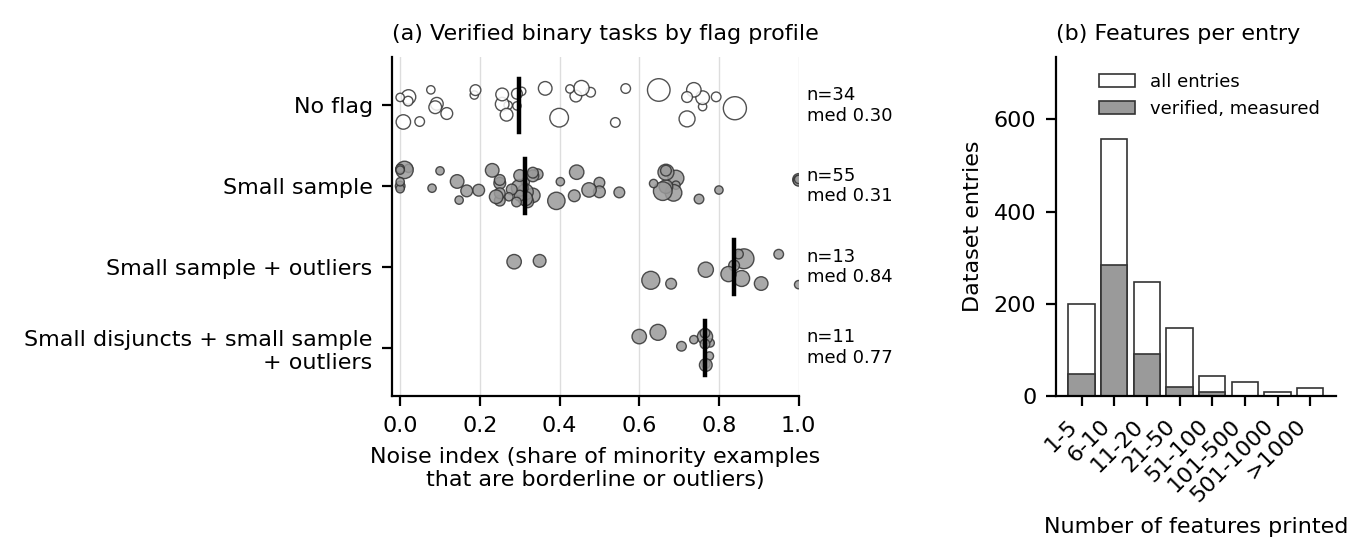
\includegraphics[width=\linewidth]{figures/data-difficulty}
\Description{Left: dot plot of the noise index (0 to 1) for 113 binary tasks in four rows by flag profile, with medians 0.30 (no flag), 0.31 (small sample), 0.84 (small sample and outliers) and 0.77 (all three flags). Right: bar chart of dataset entries by printed number of features; most entries have 6 to 10 features and none above 100 features could be verified.}
\caption{(a) Noise index of the 113 verifiable binary and binarised tasks, one row
per flag profile; marker area grows with the number of entries that use the task,
and the vertical bar marks the median. (b) Number of features printed for the
1,255 entries that report it, with the entries that could be verified and measured.
The bins are for display only.}
\label{fig:data-difficulty}
\end{figure}

The measurable part of the corpus is also low-dimensional
(Figure~\ref{fig:data-difficulty}b). The printed number of features has a median
of 9 and half of the entries lie between 4 and 10 features. The 59 entries with more
than 100 features come from 54 names in 18 papers, no name is used by more than two
papers, and none of them could be verified; the verified tasks have at most 85
features (median 9).

\claudedraft{The imbalance ratio, the one difficulty-related number most papers
print, says little about where the minority examples lie: tasks with a low ratio
can be as mixed as tasks with a high one, and a task without any flag is not
necessarily easy. Conclusions drawn from the common benchmarks speak mainly for
small, low-dimensional tables with few minority examples per feature.}

\toon{Write the interpretation in your own words. Decide whether the difficulty
profile should be reported per paper (which papers evaluate only on flag-free or
only on small-sample tasks) once the win/loss analysis resumes.}

\paragraph{Limits of the measurement.} The files come from mirrors of the
repositories (the keel-ds and imbalanced-databases packages and PMLB); for the
72 KEEL files in the official KEEL table, instance and feature counts match in
every case, and the remaining files have not yet been compared with the
repositories. PMLB stores nominal attributes as integer codes, so they enter HVDM
as numeric attributes. The labels are computed in the full feature space, not in any two-dimensional
projection.

\evidence{difficulty/verifiability\_entries.csv (643 verifiable entries, 61 papers,
131 files); difficulty/measure.py (HVDM, $k=5$, Napierala types incl.\ the rule for
rare examples) $\rightarrow$ difficulty\_measures.csv; group\_cited.py
$\rightarrow$ difficulty\_groups\_cited.csv; profile\_final.py $\rightarrow$
profile\_final\_summary.json (Table~\ref{tab:data-difficulty}); fig\_noise\_summary.json
(rank correlation); dimension\_profile.json; keel\_official\_check.csv; figure:
difficulty/fig\_manuscript.py; reported properties: out/characteristics\_coverage.json
(Analysis E).}

% ---------------------------------------------------------------------
\subsection{Where Reported Wins over SMOTE Come From}
\label{sec:data-wins}

\begin{table}[t]
\centering\small
\caption{Per-Dataset Comparisons of the Proposed Method with Plain SMOTE,
by How the Dataset Was Obtained. Wins, ties and losses compare printed values
under interim rule A (one metric fixed per paper; equal at the printed precision is a tie);
scores are not comparable across papers. KNNOR's single row, a mean over its 19 datasets,
is not a per-dataset comparison and is reported in the text instead.}
\label{tab:wins-by-type}
\begin{tabular}{lrrrrr}
\toprule
How obtained & Rows & Papers & Proposed wins & SMOTE wins & Ties\\
\midrule
Original & 166 & 26 & 132 & 29 & 5\\
Repository-defined & 119 & 9 & 90 & 13 & 16\\
Modified & 143 & 14 & 109 & 30 & 4\\
Synthetic & 5 & 1 & 5 & 0 & 0\\
Cannot be told & 105 & 13 & 83 & 9 & 13\\
Result row not matched to a dataset & 3 & 2 & 1 & 1 & 1\\
\addlinespace
All & 541 & 30 & 420 & 82 & 39\\
\bottomrule
\end{tabular}
\end{table}

At the paper level, 44 of the 73 papers use plain SMOTE as a baseline,
13 use SMOTE inside a wrapper, and 16 do not compare with SMOTE at all.
Fewer papers give rows that can be compared: 30 papers print per-dataset
scores for both the proposed method and plain SMOTE in the same table, giving
541 comparisons (Table~\ref{tab:wins-by-type}). In these, the
proposed method wins in 420 rows, ties in 39 and loses in 82.
KNNOR~\pcite{islam2022knnor} prints only a mean over its 19 datasets
(G-score .8363 for KNNOR and .8238 for SMOTE); we report it here as an
aggregate result and do not count it as a per-dataset comparison.

Comparisons with SMOTE inside a wrapper are kept apart and are not pooled
with Table~\ref{tab:wins-by-type}: all 13 wrapper papers print per-dataset
pairs, giving 293 rows. In one of them, RBBoost~\pcite{diezpastor2015randombalance},
the extracted pairs do not meet the same-table rule. The scores of its
RB-Boost come from the Boosting-family table of its supplement
(Supplementary Table~11) and those of its SMOTE ensemble (ESM) from the
data-processing-family table (Supplementary Table~3). Both tables report G-mean under one protocol (J48 with Laplace
smoothing, ensembles of 100, stratified $5\times2$-fold cross-validation), but
the paper compares methods only within each family and never compares
RB-Boost with ESM directly. Its 86 rows, 63 of them on repository-defined
data, are kept in our data for audit and excluded from every comparison set
reported here; the other 12 wrapper papers contribute 207 rows.

Split by data type, 29 of the 30 papers include at least
one standard dataset (original or repository-defined) in the comparison, and
on these 285 standard rows SMOTE wins in 42 and ties in 21. One paper reports its per-dataset comparison with SMOTE
only on modified, synthetic or unidentifiable data (INOS~\pcite{cao2013inos}); KNNOR, whose only comparison is the aggregate above, is not counted here.
Conversely, six papers compare only on standard data (GDO~\pcite{xie2022gdo}, MC-MBRC~\pcite{ma2024mcmbrc},
MKC-SMOTE, OREM-M, SCUT~\pcite{agrawal2015scut}, SPE~\pcite{liu2020spe}).

\toon{Your hypothesis H1 lives here. Look at the shares of ``SMOTE higher''
per row of Table~\ref{tab:wins-by-type} and at the per-paper split in the
Atlas (fourth tab, wins over SMOTE by data type). What you conclude, and how strongly,
is yours; the within-paper comparison (standard vs modified rows of the same
paper) is the strongest test because it holds the paper constant.}

\claudedraft{A method that wins on unmodified standard benchmarks gives the
reader evidence that does not depend on choices the authors made about the
data. Reporting the standard and the modified datasets separately would let
readers see this directly.}

\evidence{out/verified\_outcomes.csv (smote\_kind = plain SMOTE; KNNOR's aggregate,
row 295, set aside by rule R4); counts reproduced by build/reconcile\_counts.py
(out/reconcile\_counts.json). Of the 541 rows, 3 could not be matched to a dataset
entry and 15 were matched by row order only (over all 835 rows: 4 and 22). Paper-level
baselines: out/full\_summary.json, papers, smote\_kind. RBBoost: rows 574--659;
supplement Table~3 pp.3--5 and Table~11 pp.17--18; protocol p.101 and family design
p.102 of the paper; review recorded in CROSS\_TABLE\_REVIEW of build/reconcile\_counts.py.}

% ---------------------------------------------------------------------
\subsection{Can the Reported Results Be Checked?}
\label{sec:data-verifiability}

\begin{table}[t]
\centering\small
\caption{Granularity of the Results Each Paper Reports (73 Papers)}
\label{tab:granularity}
\begin{tabular}{lr}
\toprule
Per-dataset table & 47\\
Per-dataset, partial (some datasets, metrics or classifiers only) & 8\\
Plots only & 5\\
Averages over all datasets only & 5\\
Ranks only & 3\\
No comparison with other methods & 5\\
\bottomrule
\end{tabular}
\end{table}

Of the 57 papers that use SMOTE as a baseline (44 plain, 13 wrapped), 13
give a reader no per-dataset pair of scores in the paper itself: the results
are plots (Borderline-SMOTE~\pcite{han2005borderline}, Safe-Level-SMOTE~\pcite{bunkhumpornpat2009safelevel}, Cluster-SMOTE~\pcite{cieslak2006cluster}, k-means SMOTE~\pcite{douzas2018kmeans},
GLOS~\pcite{han2023glos}), averages (G-SMOTE~\pcite{douzas2019gsmote}, CISO~\pcite{yadav2025ciso}, SplitBal~\pcite{sun2015splitbal}, QC-SMOTE~\pcite{upman2026qcsmote}), or ranks (MDO, RBO~\pcite{koziarski2019rbo},
MC-NCLWO~\pcite{tao2025mcnclwo}), and the review~\pcite{hassanat2022stop}\ compares synthetic points
rather than classifiers. A fourteenth paper, KNNOR, prints its pair of scores only
as a mean over its datasets.

Baseline results are also reused across papers. QC-SMOTE copies its baseline
numbers from the VS-SMOTE paper~\pcite{qiu2025vssmote}, and every SMOTE-all value in MC-CCR's Table~6
is identical, to two decimals and on all 20 datasets, to the SMOTE-all
column of MC-RBO's Table~VI, from the same group and with the same C5.0 setup.
The same pattern appears across research groups: the Baseline, SSMOTE, GCS,
ABNC, OSMOTE and AMDO columns of EMDO's Table~5~\pcite{yao2021emdo} repeat, value for value on all
nine shared datasets, the MAUC results of AMDO's Table~6~\pcite{yang2018amdo}; EMDO states that it
uses the same datasets as AMDO but not that the baseline results were copied.
\claudedraft{Reusing a baseline is efficient, but unless it is stated, a reader
cannot tell whether the comparison was run under identical conditions.}
Several of these papers place per-dataset results on GitHub or in material
outside the paper. Where only ranks are given, the paper's own table can
still be informative: in RBO's Table~2 (CART, no added noise) SMOTE has the
better mean G-mean rank, and CISO reports itself statistically equivalent to
SMOTE.

\claudedraft{For these papers the headline claim cannot be falsified from what
is published. This does not mean the claims are wrong; it means a reader
cannot tell whether an average improvement comes from consistent gains or
from large gains on a few datasets.}

\evidence{out/full\_summary.json granularity and per-paper notes; MC-RBO
Table VI p.10 vs MC-CCR Table 6 p.10 (ai-draft/full/MC-RBO.json notes).
MWMOTE Table 5 audit: of 15 checkable rows, minority counts exact in 13, four
rows with wrong N or majority (single paper, case only).}

% ---------------------------------------------------------------------
\subsection{Recommendations for Reporting Data}
\label{sec:data-recommendations}
\begin{enumerate}
\item Name the repository and version of every dataset, and whether the full
      set or a training file was used.
\item State which class or classes form the minority and why, in the text and
      not only in a table.
\item Declare every modification (binarisation, class merging,
      undersampling, noise, dropped attributes) in the data section.
\item Give the imbalance-ratio formula, not only its values.
\item Report per-dataset results for the proposed method and plain SMOTE,
      and report standard and modified datasets separately.
\item Separate tuning datasets from evaluation datasets, as CISO and LS~\pcite{cieslak2008ls} do,
      and run the baselines rather than copying their numbers.
\item \claudedraft{Report at least one measure of where the minority examples lie
      (for example the shares of safe, borderline, rare and outlier examples) next to
      the imbalance ratio.}
\end{enumerate}

\toon{Keep, cut or reword; each item should point back to a finding above.}
